\chapter{Liste des théologiens}
% ToC of the main sections
\startcontents[mainsections]
\printcontents[mainsections]{l}{1}{\section*{Liste des théologiens et islamologues}\setcounter{tocdepth}{4}}
 



\section{Théologiens Classiques Musulmans}

%------------------------------------------------------------
\subsection{al-Ġazālī}

le joyau d'al-Ġazālī~: \emph{Le Tabernacle des Lumières}, traduit
par Deladrière, Paris, Seuil, texte très dense et très profond aux
implications nombreuses.
\cpageref{theol:AlGazali1,theol:AlGazali4,theol:AlGazali5,theol:AlGazali6,theol:AlGazali7,theol:AlGazali9,theol:AlGazali10,theol:AlGazali11,theol:AlGazali13,theol:AlGazali14,theol:AlGazali16,theol:AlGazali17,theol:AlGazali18,theol:AlGazali19,theol:AlGazali20,theol:AlGazali21,theol:AlGazali22,theol:AlGazali23,theol:AlGazali24}
\pageref{theol:AlGazali29}
\pageref{theol:AlGazali2}
\pageref{theol:AlGazali3}
\pageref{theol:AlGazali8}
%\pageref{theol:AlGazali31}
\pageref{theol:AlGazali25}
%theol:AlGazali31,theol:AlGazali32,theol:AlGazali33,theol:AlGazali34,theol:AlGazali35,theol:AlGazali36,theol:AlGazali37,theol:AlGazali38} 
%\label{theol:AlGazali1}




%------------------------------------------------------------
\subsection{Ibn Taymiyya}


 

C'est le très grand penseur (controversé) du 13\textsuperscript{ème}
siècle. Un certain nombre de ses ouvrages ont été traduits (souvent mal,
je sélectionne les meilleures traductions).


\emph{La lettre de Palmyre} traite de deux questions théologiques~: les
attributs divins et la prédestination~!

%\includegraphics[width=0.3\textwidth]{Images/image26.png}
\begin{marginfigure}
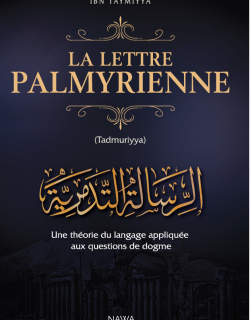
\includegraphics[width=\textwidth]{Images/image026.png}
\end{marginfigure}

-~Ibn Taymiyya, \emph{Réponse Raisonnable aux Chretiens ?} édité,
traduit et commenté par Laurent Basanese, sj., Ifpo, 2011.

-~Ibn Taymiyya, \emph{Musique et danse selon Ibn Taymiyya}: Le livre du
\emph{Samâ°} et de la danse (\emph{Kitâb al-Samâ° wa l-Raq.s}), Paris,
Vrin, 2000.

-~Ibn Taymiyya, \emph{Pourquoi les savants divergent,} Al-Hadith
éditions, 2012


Voir p. \pageref{ibn-taymiyya}.


%------------------------------------------------------------
\subsection{Ibn Toumart}
\label{IbnToumart}
\mn{E.B., « Ibn Toumart », in 23 | Hiempsal – Icosium, Aix-en-Provence, Edisud (« Volumes »,
no 23) , 2000 \url{http://
encyclopedieberbere.revues.org/1629}}


Ibn Toumart est la personnalité religieuse et politique la plus marquante du Maghreb au
XIIe siècle. Fondateur du mouvement almohade*, il devait préparer la revanche des Sanhadja
montagnards contre l’empire déjà vacillant des Almoravides. Bien que ses disciples aient
manipulé sans vergogne sa généalogie pour le rattacher à la descendance du Prophète et en
faire, donc, un chérif, il est sûr qu’Ibn Toumart était issu d’une tribu du Sous, celle des Hergha,
appartenant au groupe montagnard des Maçmouda.
 L’un de ses premiers disciples, le pieux el Baïdaq, se fit son chroniqueur et grâce à son
récit, souvent dithyrambique, il est possible de saisir l’évolution spirituelle de celui qui
devait mériter le titre de Mahdi Almohade et le qualificatif d’Impeccable. Célèbre dès son
adolescence, pour son zèle religieux et son érudition qui lui avait fait donner le surnom d’asufu
(le tison, le flambeau, en berbère), Ibn Toumart quitta un beau jour son village d’Igliz et
ses montagnes pour compléter, en Orient, sa connaissance de l’islam et jeter les bases d’une
réforme radicale.
 Son séjour en Espagne n’est pas assuré, mais demeurent des concordances étroites entre
les textes d’Ibn Hazm et ses propres propositions. En revanche, sa présence à Bagdad est
pleinement confirmée, alors que son passage à Damas est peut-être légendaire et les entretiens
qu’on lui prête avec Ghazali certainement inventés.
 Dix ans après son départ d’Igliz, Ibn Toumart entreprend un long voyage de retour au Maghreb,
au cours duquel il multiplie les étapes, passant par Alexandrie, Tripoli, Mahdia, Tunis,
Constantine et Béjaia. Sa condamnation des moeurs citadines relâchées provoque souvent des
échauffourées. A Béjaia, ses violences verbales déclenchent la fureur populaire contre lui. Le
sultan hammadite, qui l’avait d’abord bien accueilli, lança ses sicaires à sa poursuite, mais Ibn
Toumart trouva refuge dans la tribu voisine, celle des Beni Urigol, dans le village de Melala.
\paragraph{
La doctrine almohade}
 Ibn Toumart y élabore sa doctrine et réunit ses premiers disciples. Le plus cher à son coeur,
celui qu’il considère comme l’homme providentiel qui doit lui succéder, est Abd el Moumen,
le fils d’un potier de Nédroma (Algérie occidentale). El Baïdaq nous a laissé le récit émouvant
de la désignation du futur calife. Le réformateur proclama un soir en prenant sa main : “La
mission sur laquelle repose la vie de la religion ne triomphera que par Abd el Moumen ben Ali,
le flambeau des Almohades.” Celui-ci, en pleurant, dit avec humilité : “Ô Maître, je n’étais
nullement qualifié pour ce rôle, je ne suis qu’un homme qui cherche ce qui pourra effacer ses
péchés.” – “Ce qui te purifiera de tes péchés, répondit Ibn Toumart, ce sera précisément le rôle
que tu joueras dans la réforme de ce monde.”
 Une conversation avec deux pèlerins de l’Atlas qui passaient par Bougie est l’occasion du
départ des premiers Almohades vers le Maghreb el Aqsa. La petite troupe, d’une dizaine de
personnes, gagne Marrakech non sans avoir semé la bonne parole et causé quelques troubles
dans les villes traversées : Tlemcen, Oujda, Taza, Fès, où Ibn Toumart se fait remarquer par
le saccage des magasins des marchands de musique, contre lesquels il semble avoir eu une
aversion certaine. Il réitère à Marrakech, brisant à coups de bâton instruments de musique
et jarres de vin, pourchassant sous les huées la soeur de l’émir almoravide, qui chevauchait
dévoilée dans les rues de la capitale.
 Après la prise de Tin Mel (1123), il se proclame Mahdi et, de retour dans les tribus Masmouda,
ses frères de race, il organise solidement la communauté almohade avec un soin et une
connaissance des hommes qui font de ce clerc un grand homme d’État. Il crée un véritable
État montagnard, solidement organisé, disposant d’une armée fanatisée chargée de répandre
la doctrine almohade jusqu’en Ifriqiya et en Espagne.

Nous retrouvons dans cette réforme la même tendance innée vers le rigorisme moral et la
simplicité doctrinale que nous ont révélés tous les schismes et hérésies nés en Berbérie à travers
les siècles.
Dans la condamnation absolue des richesses de ce monde et de ses frivolités, c’est la voix
d’Ibn Toumart qui tonne, mais elle fait écho à celle, non moins véhémente, de Tertullien. La
lente marche des Berbères vers le Dieu unique semble ici se parachever dans la proclamation
de l’Unicité absolue de Dieu, dont Ibn Toumart rejette jusqu’aux adjectifs (le Puissant,
le Miséricordieux, le Victorieux) que lui dorment les musulmans, parce qu’ils risquent de
faire apparaître comme divisible la puissance divine. La conséquence inévitable de la toutepuissance
de Dieu ainsi comprise est la prédestination de tous les êtres créés : chacun doit
attendre dans la soumission totale ce qui lui a été assigné de toute éternité.
Cette forme de l’islam ne peut qu’être fanatique, elle ne supporte ni relâchement des moeurs,
ni relativisme dans le dogme, ni présence d’Infidèles.
11 Ces données concordaient trop bien avec l’intransigeance fondamentale des Berbères pour ne
pas aboutir : aussi, sous Abd el Moumen, le raz de marée almohade balaya le Maghreb de
toute impureté. C’est alors, semble-t-il, que disparurent les dernières communautés chrétiennes
autochtones.
\paragraph{L’État almohade}
Respectueux des traditions tribales des Berbères du Haut Atlas, Ibn Toumart organisa son
gouvernement en établissant une hiérarchie entre différents conseils imités des assemblées
tribales. Au sommet siège le Conseil des Dix, qui sont les premiers et les plus fidèles
compagnons (Abd el-Moumen*, Abou Hafs Omar*, El Bachir...). Au-dessous du Conseil
des Dix, le Conseil des Cinquante est composé de contribules d’Ibn Toumart, des Hergha et
d’autres Maçmouda de Tin Mel ou des Hintata. Les différentes tribus de la montagne étaient
ainsi représentées dans ce Conseil dont les pouvoirs étaient restreints.
Toute la société almohade était strictement hiérarchisée. A l’intérieur des groupements
ethniques apparaissait une autre hiérarchie, fondée sur les fonctions exercées, depuis celles
des compagnons les plus proches jusqu’à celles confiées aux abid (serviteurs noirs). Au
sommet de la pyramide, le Mahdi tenait solidement les rênes d’un pouvoir absolu. Cette
domination reposait sur une logique implacable : tout Almohade suspecté de tiédeur risquait
l’élimination : ainsi lors de la “journée du tri” plusieurs milliers d’almohades “infidèles” furent
massacrés. C’est par de telles actions qu’Ibn Toumart réussit à construire l’État almohade et à
assurer la naissance de la nouvelle dynastie moumenide. Seuls le prestige et la volonté d’Ibn
Toumart réussirent à faire admettre Abd el-Moumen comme le successeur désigné du Mahdi.
Encore fut-il nécessaire de cacher la mort de celui-ci pendant plus de deux ans avant de faire
reconnaître le nouveau souverain par les Cheikhs almohades.
\paragraph{références}
voir p. \cpageref{theol:IbnTumart1}


%------------------------------------------------------------
\subsection{Autres théologiens classiques}

%------------------------------------------------------------
\paragraph{Ibn Hanbal}

voir p. \pageref{Theol:IbnHanbal1}


 \paragraph{Ibn Hazm} \label{Theol:IbnHazm}{Ibn Hazm est un théologien andalou de Cordoue mort en 456H / 1064 dont
la famille s'était convertie à l'islam quelques deux siècles auparavant.
Il est à la fois poète, théologien, philosophe, historien. Son œuvre
comprend près de 400 ouvrages dont le fameux \emph{Collier de la colombe
sur l'amour et les amants}, où il aborde sous forme d'anecdotes les
manifestations et signes de l'amour. Ses analyses psychologiques sont
d'une grande finesse et s'appuient sur une perspective platonicienne où
l'amour est vu comme union des âmes à la lumière du principe de la
ressemblance. En droit, c'est un ẓahirite (extérioriste, littéraliste).
Il est très méfiant à l'égard de l'utilisation de l'analogie ou de
l'opinion~: pour lui, on doit respecter le texte dans sa littéralité. Il
a rédigé un \emph{Traité sur les religions et les écoles de pensée}. }

voir p. \pageref{Theol:IbnHazm1}, \pageref{Theol:IbnHazm2} - Polémique de Ratisbonne avec Benoit XVI.
%------------------------------------------------------------
\paragraph{Ibn Salah}
Ibn Salah
\pageref{Ibnsalah1}
%------------------------------------------------------------
\paragraph{Ibn Khaldūn}
Le penseur andalou Ibn Khaldūn \pageref{theol:IbnKhaldun} 
%------------------------------------------------------------
\paragraph{Ibn Qutayba}
Ibn Qutayba -- si ce nom ne vous est pas encore familier, cela devrait
faire `tilt' car nous l'avons rencontré au début de cette leçon. Il a
écrit un Traité sur comment rendre compte et comprendre les divergences
dans le \emph{ḥadīṯ.} A-t-il été traduit en français~? La réponse est en
note 3 --
\pageref{Theol:IbnQutayba1}
%------------------------------------------------------------
\paragraph{Kalābāḏī}
  est un auteur persan, mort aux environs de 990. Cet ouvrage
cherche à réconcilier le soufisme et l'orthodoxie. 
\pageref{theol:Kalabadi}




%------------------------------------------------------------
\section{Philosophes des Lumières}
%------------------------------------------------------------
\paragraph{Al Kindi}  \mn{\cite{PolDroit:voyage}}
%------------------------------------------------------------
\paragraph{Al Farabi}
%------------------------------------------------------------
\paragraph{Avicenne}




%------------------------------------------------------------
\section{Théologiens modernes}

%-------------------------------------------------
%------------------------------------------------------------
\paragraph{ʿAlī Ṭanṭāwī} \label{theo:AliAlTawani}
{Ali Al tantawi est originaire d'une
famille de lettrés égyptiens qui a émigré à Damas à la fin du XIXème
siècle.


Il s'est opposé à l'impérialisme occidental dans les pays
arabes et, en particulier, à la présence de la France comme mandataire
en Syrie et celle de l'Angleterre en Irak. Après l'indépendance de la
Syrie, en 1947, ses positions contre le communisme, qu'il considère
incompatible avec l'Islam lui valent d'être menacé dans son propre pays.
En 1963, il quitte la Syrie pour l'Arabie Saoudite et devient
enseignant.
Extrêmement populaire dans son pays d'adoption, il a
présenté des programmes à la radio et à la télévision pendant un quart
de
siècle.}

%-------------------------------------------------------
\label{theol:SayyidQutb}
\paragraph{Sayyid Qutb}
Sayyid Qutb (arabe :\TArabe{ سيد قطب,} Sayyid Quṭb), né le 9 octobre 1906, dans le sud de l'Égypte, et exécuté par pendaison le 29 août 1966 au Caire, est un poète, essayiste et critique littéraire égyptien, puis un militant musulman membre des Frères musulmans. Il entrera en rupture avec ces derniers à la suite du développement d'une idéologie islamiste radicale, le \textbf{qutbisme}.


Les idées de Sayyid Qutb se résument schématiquement ainsi :
\begin{itemize}
    \item 
L'islam est en crise. Les millions de gens qui se réclament de l'islam n'en comprennent en réalité pas grand-chose, ils ne sont pas de vrais musulmans. Qutb prononce donc une condamnation très forte de la société égyptienne contemporaine.
  \item 
Un retour aux vraies valeurs de l'islam est nécessaire. Malheureusement les masses populaires manipulées par le nassérisme sont incapables de s’en sortir. Il appartient donc à une élite de guider les masses en jouant le même rôle que celui des compagnons du prophète de l'islam; cette élite qu'il appellera dans plus d'un ouvrage "\textit{annawâte assoulba}" (littéralement "le noyau dur"). Le but est de réislamiser la société.
  \item 
L'islam apporte une solution complète à tous les problèmes, politiques, économiques, sociaux. En revanche, les influences occidentales sont dangereuses et nuisibles. Il dénie le qualificatif de « civilisation » (notamment dans son livre Mushkilât al-hadâra : Problèmes de la civilisation) aux blocs de l'est (socialiste) et de l'ouest (capitaliste), qu'il renvoie dos à dos comme représentant deux faces d'une même entité qu'il qualifie de \textit{Jahiliya} (ignorance). Ce terme, qui renvoie à la période précédant l'islam durant laquelle l'Arabie était polythéiste et ignorante donc du vrai Dieu, a une forte connotation négative dans l'imaginaire musulman.
  \item 
L'idée d'une « lutte contre les Juifs » fut aussi présente dans la pensée de Sayyid Qutb, qui écrivit au début des années 1950 l'opuscule \textit{Notre combat contre les Juifs}. Dans son commentaire de la sourate 5, Sayyid Qutb réaffirmera l’accusation : « Depuis les premiers jours de l’islam, le monde musulman a toujours dû affronter des problèmes issus de complots juifs. (…) Leurs intrigues ont continué jusqu’à aujourd’hui et ils continuent à en ourdir de nouvelles. » 
\end{itemize}


%------------------------------------------------------------
\section{Théologiens et Islamologues contemporains}
%------------------------------------------------------------
\paragraph{Tarik Ramadan}
 \begin{itemize}
  \item Paradoxe de Tarik Ramadan~: dire que le radicalisme vient de
    l'occident. Et ensuite, valoriser le communitarisme pour refuser les
    coutumes locales et en particulier celles de la laicité.
  \end{itemize}
  
Voir réflexion sur le moratoire.
Voir p. \pageref{Theol:TRamadan1} (connaissance en France).

%------------------------------------------------------------
\paragraph{Mohammed Arkoun}
 Mohammed Arkoun (arabe  \TArabe{ : محمد أركون, } 1928 Algérie, mort en 2010 à
Paris, est un intellectuel algérien qui s'inscrit dans la tradition des
Lumières françaises, historien, islamologue et philosophe. Parmi ses
sujets de prédilection, l'impensé dans l'islam classique et
contemporain. humaniste, laïque, un militant actif du dialogue entre
les religions, les peuples et les hommes. Spécialiste de l'islam, il
plaidait pour un islam repensé dans le monde contemporain. Il y a
consacré de très nombreux ouvrages dont La Pensée arabe (Paris, 1975),
Lectures du Coran (Paris, 1982), Penser l'islam aujourd'hui (Alger, 1993)
Savant à la pensée profonde, c'était également un intellectuel engagé. Son analyse serrée des processus à l’œuvre dans l’islam d’hier était indissociable de ses appels répétés à une réforme des sociétés islamiques contemporaines. Il n’a cessé de porter ce message dans les divers colloques où il était convié, y compris là où l’on ne s’attendrait guère à croiser un islamologue : à un congrès de psychanalystes lacaniens, dans des conférences sur la condition féminine…
Il a choisi de consacrer les dernières années de sa vie à retravailler les textes issus de ces rencontres. Traitant de la nécessité de la réforme, voire de la « subversion » de l’islam, de l’ouverture lacanienne à la parole et à la « raison émergente », de la condition féminine en islam ou encore du rapprochement entre sunnites et shî‘ites, ils montrent combien la pensée de Mohammed Arkoun est plus que jamais féconde pour penser notre époque.
Voir  \cpageref{theol:Arkoun1,theol:Arkoun2,Theol:Arkoun4} 
\label{theol:Arkoun3}
%------------------------------------------------------------
\paragraph{Rachid Benzine}.
Islamologue et historien, Rachid Benzine s’est intéressé à ces questions après sa rencontre avec le prêtre catholique Christian Delorme à Lyon et a beaucoup travaillé avec des théologiens protestants.
%------------------------------------------------------------
\paragraph{Pierre Lory}
\label{Theol:PierreLory}
Un des grands connaisseurs de Qušayrī est
Pierre Lory.

Même en dehors des cercles salafistes, nombreux sont aujourd'hui les
musulmans~

\begin{cite}
« qui voudraient que le Coran soit un discours unique,
et qui se méfient des interprétations différentes les unes des autres
»,~
\end{cite}
\emph{}déplore~{{Pierre
Lory}}. Cet islamologue a contribué au récent site {{Coran 12-21}}
Internet~\url{https://coran12-21.org/fr/} , qui
présente différentes versions du Coran, dans trois langues différentes.

Pour lui, comme pour d'autres spécialistes, considérer le Coran comme un
tout dogmatique et intouchable est non seulement dangereux, mais aussi
erroné.

%------------------------------------------------------------
\paragraph{Abdessamad
Belhaj}
\begin{cite}
« La lecture littérale est en elle-même une
interprétation, puisqu'elle est fondée sur la prémisse que les propos du
Coran sont généralisables et peuvent faire fi des circonstances
particulières »,~
\end{cite}
remarque
l'islamologue~{\underline{Abdessamad
Belhaj}}, chercheur au Centre interdisciplinaire d'études de l'islam
dans le monde contemporain de l'Université catholique de Louvain.

%------------------------------------------------------------
\paragraph{Abdel Wahhab Meddeb}
{Meddeb est
    un penseur tunisien}, professeur à la Sorbonne en littérature
    comparée, il a animé des années durant l'émission Culture d'islam
    sur France culture. Il est décédé le 6 novembre 2014.






%----------------------------------------------------------------------------------------------------
\section{Islamologie Catholique}

\mn{intègre les notes de la conférence d’Emmanuel Pisani aux AIDEO le 15 nov 2021 pour les 100 ans de la thèse de doctorat de Louis Massignon}

% ------------------------------------------------------
\subsection{Tendances polémistes}
Si la tendance Massignonienne s’est imposée pour Vatican II, une tendance plus polémiste a toujours existé. Contrairement à Massignon, il montre le côté radical de la différence des deux religions.  
% ------------------------------------------------------
\paragraph{Henri Lammens} jésuite. Voir \href{https://fr.wikipedia.org/wiki/Henri_Lammens}{lien wikipedia}.

Voir : p. \pageref{Theol:Lammens2} et p. \pageref{Lammens1}.
% ------------------------------------------------------
\paragraph{Edouard Marie Gallez}. Il rattache l'origine de l'islam au judéo-nazaréisme, dont il serait dérivé.

% ------------------------------------------------------
\subsection{une vision de l’Islam au delà des stéréotypes}

 le  « décentrement mental à la Copernic » de Massignon. 
\begin{Ex}
Alors même que l’Islam se déclare la religion monothéiste par excellence, la chanson de Roland identifie l’Islam à trois dieux. 
\end{Ex}
L’abbé Pierre x (?) se fait moins polémique et apologétique au fur et à mesure du temps. Les premiers islamologues catholiques est la recherche pour renouveler le regard catholique de l’Islam. Sous l’impulsion du \emph{ Baron Carra de Vaux}, qui publie des ouvrages grand public sur des figures de l’Islam. Veut sortir des fables et grossieretés. Une vision équilibrée qui permet un jugement juste de l’Islam. Cela n’a pas la critique historique allemande mais structuré et erudit (5 volumes).  Dans son avant propos : « mieux comprendre l’Orient,… alors même que la France est un vaste empire en Islam ».  Abdel Jadid (?) converti, professeur à l’ICP, contribuer aux développements arabisants en France. 

\paragraph{Louis Massignon}

L’islamologue Massignon s’est avant tout situé dans la grande lignée des études sur l’Islam orthodoxe, son premier souci étant de démontrer que l’Islam a une dimension mystique et que c’est l’Islam sunnite essentiellement qui se prête à cette dimension. Mais que ce soit à travers son thème de recherche principal, Ḥallāğ, ou dans le reste de son œuvre, dans ses cours au Collège de France et à l’École des Hautes Études, dans ses incessants déplacements en Iran, en Syrie, au Liban, il s’est heurté au šī‘isme à tous les carrefours.

Massignon, \emph{l’islamologie catholique}, a transformé la vision de l’Islam. C’est un converti au catholicisme. il fait l’expérience de Dieu sur cette terre d’Islam (voir p. \pageref{fig:Ctesiphon}). Il se sent redevable de l’Islam pour sa conversion. Sa thèse, la passion d’Hallag : dans ce spirituel de Bagdad, il découvrit d’un musulman : 
\begin{quote}
Mais vous aimez, … nous aimons n’importe quoi… on n’aime pas Dieu… mais il y a un musulman mystique mort sur la croix pour l’amour de Dieu, c’est Hallag.
\end{quote}

{Mansur al-Ḥallāğ pour Massignon} figure du Christ de l'Islam.

  Dieu demande à toutes les créatures devant l'homme. Une créature
  refuse. Traditionnellement, c'est considéré comme un refus
  d'obeissance de l'ange (c'est de la boue puante~»). Pour al Hallaj
  c'est uniquement devant Dieu et c'est une épreuve de Dieu, c'était
  révélé à l'ange ce qu'est Dieu. Dieu est dans l'homme.
  \url{https://www.youtube.com/watch?v=Let1X-8zsXU\&t=1428s}
  C'est à cause de cette divinisation qu'il sera condamné, hétérodoxe.



% ------------------------------------------------------
\subsection{ islamologie selon les catégories catholiques}.
Ici les kalam et Hadith, à la lumière des catégories catholiques. Théologie comparée. 

\paragraph{P. Anawati}
1947,  le frère Louis Gardet, \sn{1904-1986} et le Père Anawati (dominicain), \emph{introduction à la théologie musulmane, essai de théologie comparée}. A la lumière de S. Thomas d’Aquin, la grâce, la sur-nature,… qu’ils comparent l’Islam à ces catégories. Qualité de l’irudition mais à qui cela s’adresse. Plusieurs difficultés : fin du thomisme, et travaux sur les lectures des sources islamiques : « ce n’est pas faux mais ce n’est pas cela ». il ne prend pas assez en compte la singularité de la langue arabe (catégorie thomisme). « Par trop dogmatisant en ne prenant pas en compte la grammaire et les racines arabes ».  Massignon disait, par opposition, avait renoncé à un cours écrit pour un cours spontané, révolution pédagogique. « pour apprendre la pensée ; apercevoir dans le ton, l’incertitude de la pensée ». 
\paragraph{Denise Masson} traduction du Coran \sn{"Traduction du coran, c'est celle de Blachière mais en bon Français (sic)}. Essaye de montrer « monothéisme coranique et monothéisme biblique » (1976). Approche objective non apologétique. La réception de l’ouvrage est ambivalente. L’Eglise lui refuse l’imprimatur, car elle n’a pas montré la supériorité du Christianisme. Anawati émet des réserves sur le comparatisme, comme s’il était révélé et équivalent à la Bible et qu’on puisse y retrouver la plupart des mystères chrétiens. « lecture tronquée du maître, avec des catégories à la place du style poétique de Massignon ». 
% ------------------------------------------------------
\subsection{Vatican II et IDEO} Avec Vatican II, il ne s’agit pas de comparer l’Islam mais de se situer dans l’axe de l’Islam lui-même. La création de l’ISTR à la Catho : « pour que le dialogue ne soit pas une velléité, ou un monologue, mais sur le respect du message de l’Islam… Préférer l’effort de compréhension … et non de juger ». Dans ce paradigme, le dialogue des rationalités, colloque de l’ISTR en 2016

\paragraph{Opposition avec les universités d’Etat}. Dans une lettre à l’ICP, leur parler d’une lecture philosophique compatible avec leur foi et non une philosophie athée. Rendre compte des sources islamiques, présentées par les commentateurs musulmans. Mais alors quel sens catholique et quel sens critique que l’on attend de l’université ? Il manque une appréciation théologique. Lettre des étudiants… Père Douillard : « les étudiants n’ont pas répondu de façon intelligente par rapport au choc de la plongée dans l’étude des autres religions ». Emilio Platti : attitude existentielle fondamentale. Toute compréhension d’Islam devrait impliquer cette attidude existentielle. 
 4ème dimanche de juillet. Pèlerinage en Bretagne avec la sourate la Caverne / un pardon breton mélé d’islam (les 7 dormants d’Ephèse). Regard renouvelé pour le dialogue. Périguene : Islam et christianisme : deux grandeurs appelés à se parler et se rencontrer.   Fonder le dialogue religieux en se positionnant du point de vue de l’Islam. Asseoir le point de vue musulman du dialogue : Sirai, Père blanc,… Robert Caspar. Approche ICP sur l’islamologie. « l’apostasie en Islam », « pluralisme religieux en Islam ». Ces islamologues catholiques vont rechercher dans les sources de l’Islam l’extension du Fitr pour le dialogue 
\mn{N°33 MIDEO : théologie musulmane des religions. }

\paragraph{Emmanuel Pisani}
Frère dominicain et islamologue, Emmanuel Pisani est directeur de l’Institut de Science et Théologie des religions (ISTR) à l’Institut catholique de Paris.

\paragraph{Adrien Candiard}

\paragraph{Père Christian Salenson,} prêtre français, directeur de l’Institut de science et de théologie des religions de Marseille (ISTR)


\paragraph{Michel Younès}
Professeur en théologie et islamologie, il dirige le Centre d’étude des cultures et des religions. Il a codirigé le diplôme d’université, « Religion, liberté religieuse et laïcité » de 2013 à 2019. Il coordonne PLURIEL, Plateforme de recherche sur l’islam en Europe et au Liban. Coordinateur du séminaire « Religions et entreprises ».
Depuis 2020 il est directeur délégué de l’Unité de recherche « CONFLUENCE Sciences \& Humanités », UCLy
Ecrit le bulletin de Théologie des religions dans \textit{recherche de science religieuse}.

% ------------------------------------------------------
\subsection{une islamologie comme ressource pour une théologie catholique} . 

Cette fois ci , il s’agit de se laisser par les sources islamiques elles-mêmes, elles constituent une ressource pour approfondir une théologie catholique, renouvelée, inculturée en terre arabe. En 1967, l’ISTR avait fait un cours de « christianisme et Islam », Michel Ayeb : relire les écritures bibliques à la lumière du récit du prophète et du Coran. L’Islam revendique leur rattachement à Abraham.  On voit cela chez Christian de Chergé, se laissant décentrer grâce à l’Islam. Mgr Fitzgerald, les plus beaux noms divins, entrer dans le mystère des noms de Dieu puisque Dieu a refusé de donner son nom à Moise. Ramon Lul a écrit les « 100 noms divins » contre l’Islam, pour réfuter le texte islamiqu. Ce n’est pas l’approche de Mgr Fitzgerald. Approche comparative, et non comparée. En Islam, Klaus von Stosch \sn{\cite{GroesslStosch:Impeccability}} avec une approche renouvelée sur le mystère chrétien par une approche eschatologique qui est celle de l’islam. 

\paragraph{approche mystique} (Beauregard)



Dimension critique de l’islamologie peut être mal placée dans le cadre catholique. Mais cela se fait dans des facultés théologiques, où la critique / dimension réflexive est au cœur de ces facultés. Repenser dans un contexte de post modernité des débats théologiques difficiles.


\paragraph{Charles de Foucault}
Massignon a pensé suivre Charles de Foucault. Une clé pour comprendre cette fraternité universelle. \mn{Fratelli Tutti 253.}

\paragraph{Hubert de Chergé}
Lectio divina. 1ere règle de Benoit : écoute de la pensée de l’autre. 

\stopcontents[mainsections]
\section{Matériel d'Etude}\label{matuxe9riel}

\url{https://www.onelittleangel.com/livres/sacres/le-saint-coran.asp}

\url{https://coran.oumma.com/sourate/20} . Conseillé par Emmanuel
Pisani.

\url{https://www.lexilogos.com/clavier/arabe_latin.htm}

\url{https://referenceworks.brillonline.com/browse/encyclopedie-de-l-islam}

\url{https://www.lexilogos.com/coran.htm} : lexilogos y compris mot à
mot



\chapter{A trier}


\section{Notes diverses à repositionner}







Important de connaître un auteur pour avoir un avis objectif.





\begin{itemize}

  
\item  Est-ce que j'utilise la raison, l'analogie, la coutume locale ? c'est
  cela les différences.
\item  Si la coutume est la laicité, je dois en tenir compte pour mon avis.

  \begin{itemize}
  \item    Le shavinisme qui intègre le ur, la coutume,
  \item     le hanafisme, aussi~
  \item    la où on le ferait moins, c'est le hanbalisme.
  \end{itemize}
\end{itemize}



  Pour quitter l'Islam, la peine est celle de la Loi locale. En France,
  si on définit l'islam comme une loi, on dit son aversion. Tout le
  chapitre sur la loi, «~islam = loi~», est un schématisme redoutable.
  Ce n'est pas qu'un texte législatif. Malheureusement, il y a tout un
  courant dans l'Islam qui encourage cette lecture caricaturale. Dans
  les pays occidentaux, on peut combattre avec les idées l'islam
  radical.
  
  \subsection{Aristote}
  Penser raisonnablement : éviter le relativisme (l'Islam n'existe pas) mais ne pas non plus en faire une essence.
  
  \subsection{Islam compliqué}


Rachid Benzime

Islam, compliqué à lire le coran sans clé herméneutique

Passé colonial~en France~:

champ sémantique~: passer d'un champ indigène, à immigré, à ~musulman.
La religion devient le marqueur identitaire.

Pisani~:

Compliqué l'islam~; islam~: complexe

Edgar Morin~: c'est quoi la complexité d'un fait social. Si complexe,
reponse complexe

Ici, les arrières pensées~: on croit connaitre de l'islam alors que ce
n'est qu'une réalité.

Les musulmans comme «~citadelles assiégées~»

Difficile pour les musulmans de voir une certaine réalité car l'islam
quelque chose de beau.

«~un terroriste qui se dit musulman, on n'a pas le droit de lui dire
qu'il n'est pas musulman~»

Derrida~: «~il faut bien séparer l'Islam de l'Islam~».

Accepter que l'islam est pluriel, alors que l'islam est vécu par les
personnes comme unique.

Pisani~:

Macron~: l'islam est en crise.

Ce n'est pas possible pour les musulmans~: «~l'islam ne peut pas être en
crise~» - méta religieux.

Mohammed Arkoun~: le fait islamique. Dieu est absent.

Trop de représentations dans le champ «~Islam~». Mot trop chargé.

What is Islma.
